\documentclass{Controle}

\begin{document}

\nom

\section*{Morphologie externe}

%\noindent\fbox{
%\begin{minipage}{\linewidth-2\fboxrule-2\fboxsep}
%\textbf{Astuce : }pour différencier les veines des artères :
%\begin{itemize}
%\item Les veines ont une paroi fine, souple et foncée.
%\item Les artères ont une paroi épaisse, rigide et claire.
%\end{itemize}
%\end{minipage}}

\begin{figure}[ht]
\centering
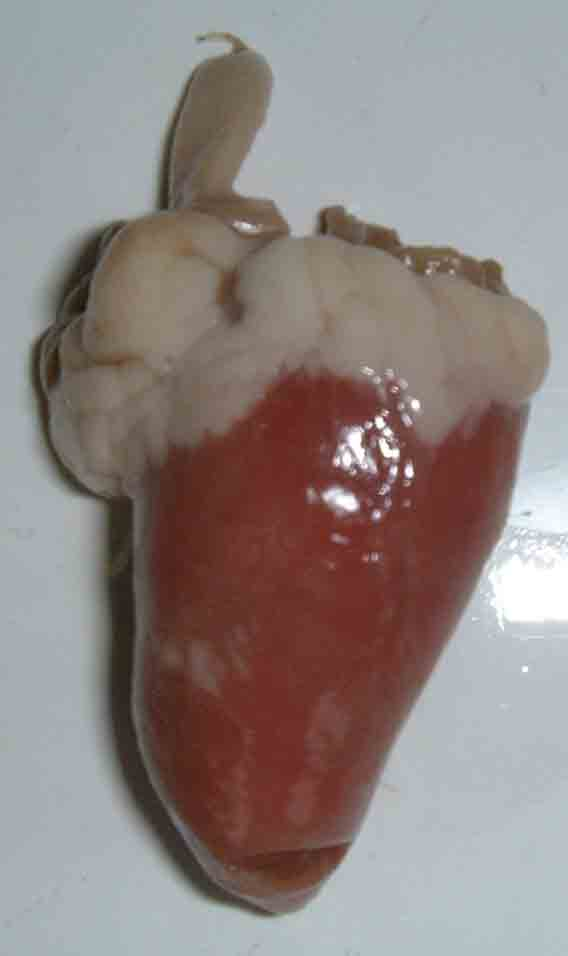
\includegraphics{coeur_poulet}
\caption{photo d'un cœur de poulet en vue ventrale. OD : oreillette droite ; CA : crosse aortique ; OG : oreillette gauche.}
\end{figure}

\question[]{Orientez le cœur dans votre cuvette comme sur la photographie. Repérez toutes les structures qui sont signalées. Appelez le professeur pour faire valider.}{1}{}{}

\section*{Expérience d'injection d'eau}

Cette expérience est réalisée à la paillasse du professeur. Elle consiste à injecter de l'eau dans le cœur et à voir par où elle ressort. Pour plus de facilité, on insère des tubes plastiques au niveau des quatre principaux vaisseaux sanguins du cœur : la veine cave, la veine pulmonaire, l'artère aorte et l'artère pulmonaire.

\question[]{Complétez le tableau suivant à l'aide de vos observations.}{4}{}{}

\tabulinesep=2mm
\noindent\begin{tabu}{|X[cm]|X[cm]|X[cm]|X[cm]|X[cm]|}
\hline
L'eau rentre par & \multicolumn4{c|}{L'eau ressort par}\\
\tabucline
\tabuphantomline
& l'artère pulmonaire & l'artère aorte & la veine cave & la veine pulmonaire\\
\hline
l'artère pulmonaire & \rule{0pt}{.5cm} & & & \\
\hline
l'artère aorte & \rule{0pt}{.5cm} & & & \\
\hline
la veine cave & \rule{0pt}{.5cm} & & & \\
\hline
la veine pulmonaire & \rule{0pt}{.5cm} & & & \\
\hline
\end{tabu}

\question{L'eau ressort-elle au hasard ?}{1}{}{}

\question{Proposez une hypothèse pour expliquer pourquoi l'eau ne ressort pas au hasard.}{1}{}{\ligne{1}}

\question{Comment peut-on vérifier votre hypothèse ?}{1}{}{\ligne{1}}

\newpage

\section*{Dissection}

Avec les ciseaux, effectue une coupe transversale (CT) au niveau des ventricules comme indiqué ci dessous sur le schéma.

\begin{figure}[ht]
\centering
%\includegraphics{CT_coeur_poulet.png}
\end{figure}

Observe la section ainsi obtenue. Repère les 2 cavités et les parois musculaires des ventricules droit et gauche.

\question{Est-ce que les deux ventricules communiquent entre eux ?}{1}{}{}

Introduis la sonde cannelée dans l’aorte et repère dans quel ventricule elle débouche. (Parfois l’artère aorte est sectionnée mais tu dois pouvoir repérer son embouchure)

Fais une coupe longitudinale du coeur (CL) en coupant avec les ciseaux le long de la sonde cannelée de l’aorte au ventricule (voir schéma suivant).

\begin{figure}[ht]
\centering
%\includegraphics{CL_coeur_poulet.png}
\end{figure}

\question[]{Complétez le schéma-bilan de la page suivante, avec les légendes :
\begin{itemize}
\item ventricule gauche,
\item ventricule droit,
\item oreillette gauche,
\item oreillette droite.
\end{itemize}}{4}{}{}

\vspace*{\stretch{1}}
\begin{figure}[ht]
\centering
\includegraphics{coeur_circulation_totale}
\end{figure}
\vspace*{\stretch{1}}

\end{document}